
\documentclass[xcolor=dvipsnames]{beamer}

\usetheme{Madrid}
\useoutertheme{miniframes} % Alternatively: miniframes, infolines, split
\useinnertheme{circles}
\usepackage{booktabs}
\newcommand{\ra}[1]{\renewcommand{\arraystretch}{#1}}

\definecolor{UBCblue}{rgb}{0.04706, 0.13725, 0.26667} % UBC Blue (primary)
\definecolor{UBCgrey}{rgb}{0.0, 0.87, 0.75} % Hatsune Miku Palette (secondary) NEON 
%\definecolor{UBCgrey}{rgb}{0.0, 0.6, 0.6} % Hatsune Miku Palette (secondary)  
%\definecolor{UBCgrey}{rgb}{0.3686, 0.5255, 0.6235} % cool neon feel w UBC blue 
%\definecolor{UBCblue}{rgb}{0.04706, 0.13725, 0.26667} % UBC Blue (primary)
%\definecolor{UBCgrey}{rgb}{0.3686, 0.999, 0.6235} % UBC Grey (secondary)

\setbeamercolor{palette primary}{bg=UBCblue,fg=white}
\setbeamercolor{palette secondary}{bg=UBCblue,fg=white}
\setbeamercolor{palette tertiary}{bg=UBCblue,fg=white}
\setbeamercolor{palette quaternary}{bg=UBCblue,fg=white}
\setbeamercolor{structure}{fg=UBCblue} % itemize, enumerate, etc
\setbeamercolor{section in toc}{fg=UBCblue} % TOC sections

% Override palette coloring with secondary
\setbeamercolor{subsection in head/foot}{bg=UBCgrey,fg=white}

\title[Meeting 2]{Journal Club: Convolutional Networks on Graphs for Learning Molecular Fingerprints (Duvenaud \textit{et al.})}
\date{May 8, 2018}
\author[Stefan O. Gugler]
{Stefan O. Gugler}
\institute[MIT]{Massachusetts Institute of Technology  \\Department of Chemical Engineering}

\begin{document}
	
\begin{frame}
	\titlepage
\end{frame}


\begin{frame}
\frametitle{Abstract}
\begin{itemize}
\item Convolutional Neural Network on graph
\item end-to-end learning of prediction pipelines
\item input: arbitrary graphs
\item generalization of circular fingerprints
\item interpretability \& performance
\end{itemize}
\end{frame}

\begin{frame}
\frametitle{State of the art}
\begin{itemize}
\item Currently: Fixed size and off-the-shelf fingerprints
\item New: Replace fingerprint with a differentiable neural network whose input is a molecular graph
\item First layers convolutional, later layers pooling
\item benefits: optimized fingerprints outperform off-the-shelf fingerprints
\item benefits: don't need 43,000 sized vector because we only use relevant features
\item benefits: notion of similarity enhances interpretability
\end{itemize}
\end{frame}

\begin{frame}
\frametitle{Circular Fingerprints}
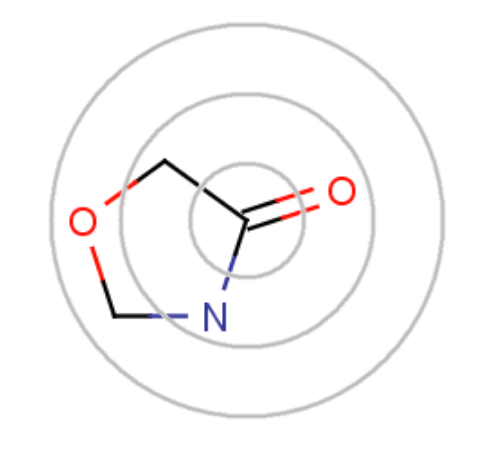
\includegraphics[width=0.2\linewidth]{img/circular1.png}
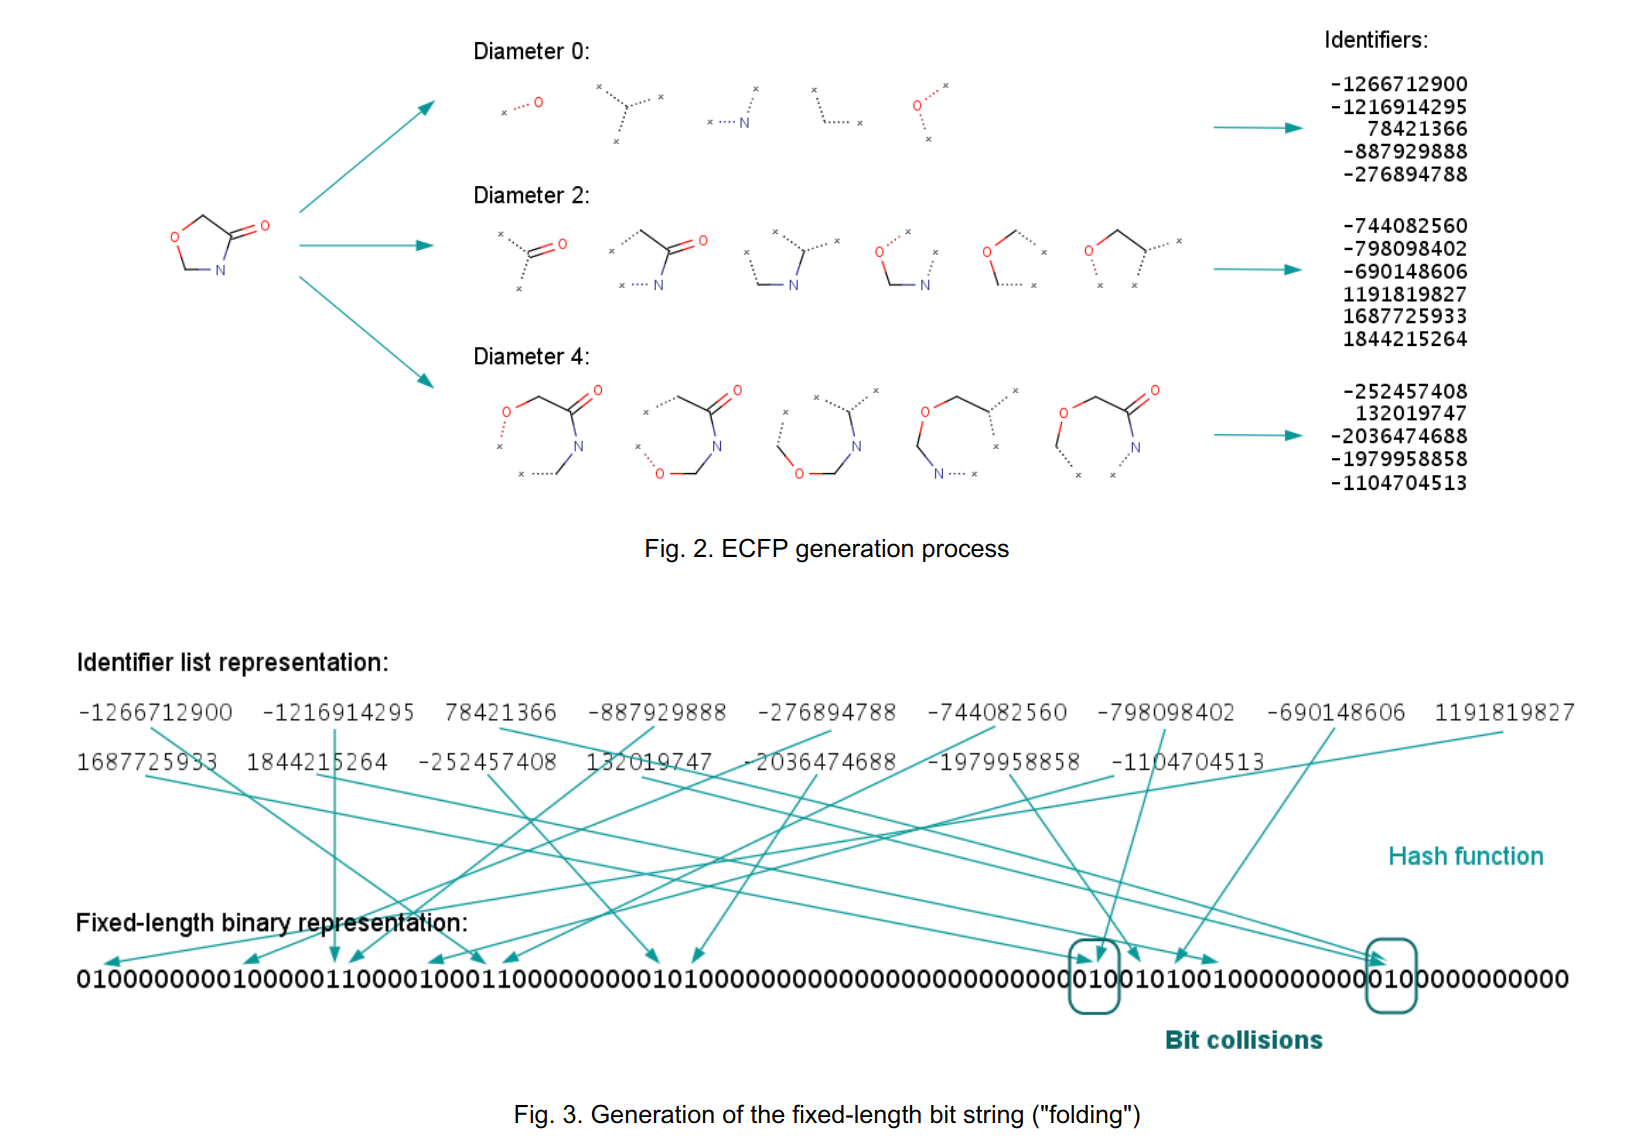
\includegraphics[width=0.8\linewidth]{img/circular2.png}
\end{frame}

\begin{frame}
\frametitle{Differentiable Fingerprints}
\begin{itemize}
\item discrete hash function $\rightarrow$ smooth NN layer 
\item indexing $\rightarrow$ softmax
\item canonicalization: sorting $\rightarrow$ permutation-invariant function like summing
\end{itemize}
Large random weights in NN fingerprints are the limit of discrete fingerprints.
\end{frame}

\begin{frame}
\frametitle{Comparison circular and neural fingerprints}
%Continuous generalization of pairwise Tanimoto distance
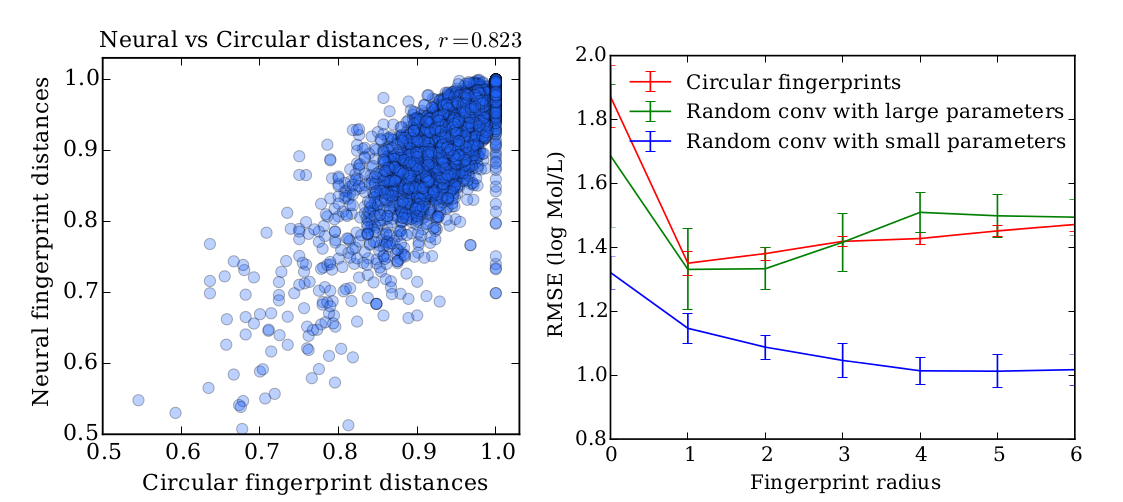
\includegraphics[width=\linewidth]{img/comp.png}
\end{frame}

\begin{frame}
\frametitle{Interpretability}
Each feature of the circular fingerprint can only be activated once, hence the long feature vector. Neural features can be activated by similar substructures, resultin gin shorter more interpretable vectors.
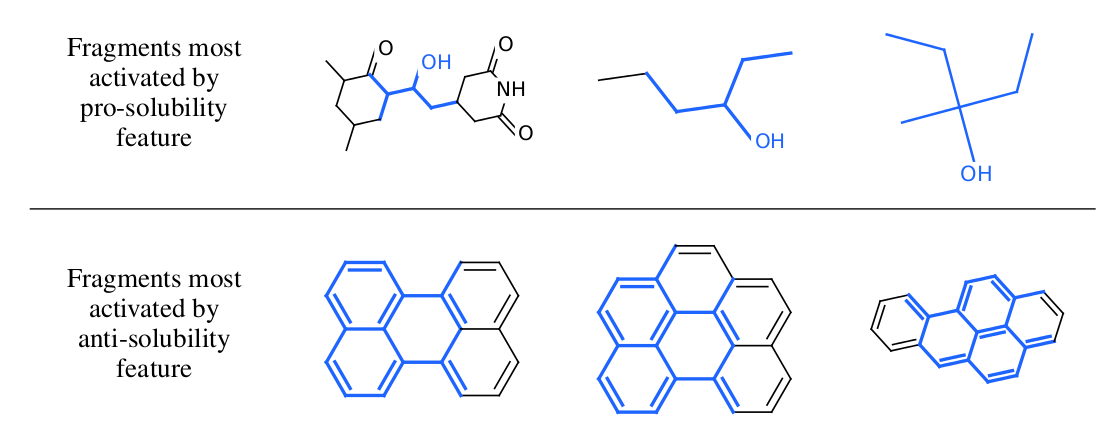
\includegraphics[width=\linewidth]{img/interpret.png}
\end{frame}



\begin{frame}
\frametitle{Predictive performance}
\begin{itemize}
\item Solubility (1,144)
\item Druf efficacy (10,000)
\item Photovoltaic efficiency (20,000)
\end{itemize}
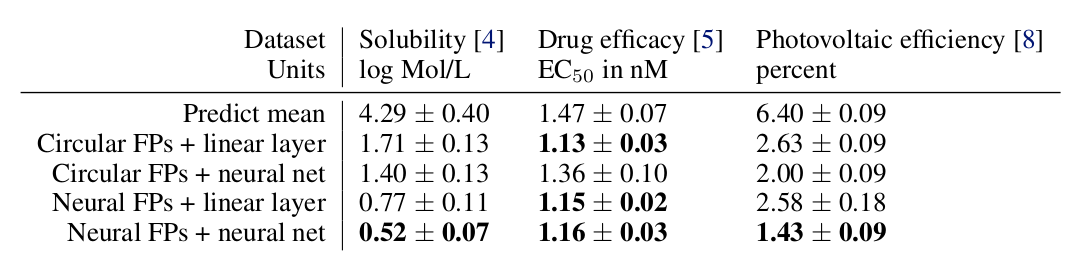
\includegraphics[width=\linewidth]{img/results.png}
\end{frame}

\begin{frame}
\frametitle{Drawbacks}
\begin{itemize}
\item Computational cost due to matrix multiplications $\mathcal{O}(\textrm{depth} \cdot \textrm{fp-length} \cdot \textrm{features} \cdot \textrm{atoms} +  \textrm{depth} \cdot \textrm{atoms} \cdot \textrm{features}^2)$
\item Information Propagation: Worst case $\frac{N}{2}$ layers to distinguish $N$ atoms.
\item Enantiomers and \textit{cis/trans} isomers not handled
\end{itemize}

\end{frame}


\end{document}